% smaller samples
\section{Analyzing Smaller Samples}
\label{sec:smallerDist}




We build a similar distribution using just 5 Tehsils (max) per province as seen in Figure~\ref{fig:fiveDist} with the code here:.
\begin{knitrout}
\definecolor{shadecolor}{rgb}{1, 1, 1}\color{fgcolor}\begin{kframe}
\begin{alltt}
pak5 <- pak[pak$Tehsil %in% \hlfunctioncall{unlist}(\hlfunctioncall{dlply}(pak, .variables = \hlstring{"Province"}, .fun = village.list, 
    num = 5, unit = \hlstring{"Tehsil"})), ]
pak5$Tehsil <- \hlfunctioncall{factor}(pak5$Tehsil)
rice5Perc <- \hlfunctioncall{build.dist}(data = pak5, lhs = \hlstring{"New_ID"}, group = \hlstring{"Province"}, question = \hlstring{"RiceLost"})
rice5Perc$Size <- \hlstring{"5"}
compare5 <- \hlfunctioncall{compare.dist}(ricePerc, rice5Perc, by = \hlfunctioncall{c}(\hlstring{"Province"}, \hlstring{"RiceLost"}))
compare5$Partial.Size <- \hlfunctioncall{impute.col}(col = compare5$Partial.Size, 5)
\hlfunctioncall{ggplot}(rice5Perc, \hlfunctioncall{aes}(x = RiceLost, y = Percent)) + \hlfunctioncall{geom_bar}(stat = \hlstring{"identity"}) + 
    \hlfunctioncall{facet_wrap}(~Province) + \hlfunctioncall{opts}(axis.text.x = \hlfunctioncall{theme_text}(angle = 90))
\end{alltt}
\end{kframe}
\end{knitrout}


\begin{figure}[!hbt]
\begin{knitrout}
\definecolor{shadecolor}{rgb}{1, 1, 1}\color{fgcolor}\begin{kframe}


{\ttfamily\noindent\textcolor{warningcolor}{\#\# Warning: 'opts' is deprecated.\\\#\# Use 'theme' instead.\\\#\# See help("Deprecated")}}

{\ttfamily\noindent\textcolor{warningcolor}{\#\# Warning: 'theme\_text' is deprecated.\\\#\# Use 'element\_text' instead.\\\#\# See help("Deprecated")}}\end{kframe}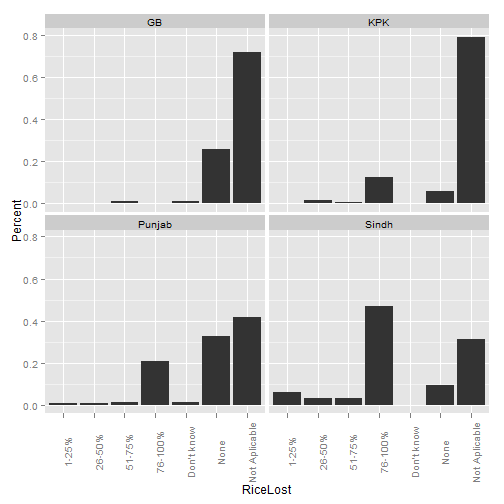
\includegraphics[width=.9\linewidth]{smallerDist/figures/fiveDistPlot} 
\end{knitrout}

\caption{Distribution for five Tehsils per Province.\label{fig:fiveDist}}
\end{figure}

The same distributions for 10 and 15 samples are seen in Figures~\ref{fig:tenDist} and \ref{fig:fifteenDist} respectively.  This time, for brevity, the code will not be displayed.

\begin{figure}[!hbt]
\begin{knitrout}
\definecolor{shadecolor}{rgb}{1, 1, 1}\color{fgcolor}\begin{kframe}


{\ttfamily\noindent\textcolor{warningcolor}{\#\# Warning: 'opts' is deprecated.\\\#\# Use 'theme' instead.\\\#\# See help("Deprecated")}}

{\ttfamily\noindent\textcolor{warningcolor}{\#\# Warning: 'theme\_text' is deprecated.\\\#\# Use 'element\_text' instead.\\\#\# See help("Deprecated")}}\end{kframe}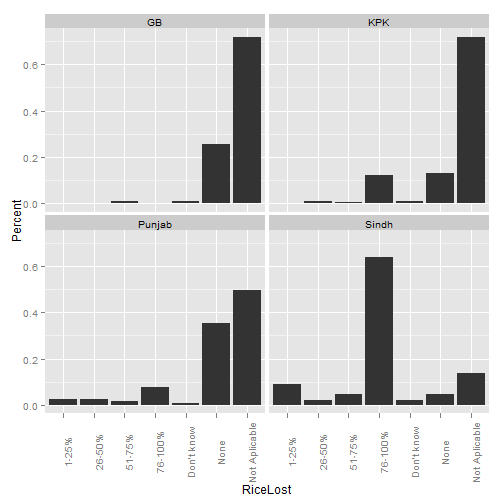
\includegraphics[width=.9\linewidth]{smallerDist/figures/tenDist} 
\end{knitrout}

\caption{Distribution for ten Tehsil per Province.\label{fig:tenDist}}
\end{figure}

\begin{figure}[!hbtp]
\begin{knitrout}
\definecolor{shadecolor}{rgb}{1, 1, 1}\color{fgcolor}\begin{kframe}


{\ttfamily\noindent\textcolor{warningcolor}{\#\# Warning: 'opts' is deprecated.\\\#\# Use 'theme' instead.\\\#\# See help("Deprecated")}}

{\ttfamily\noindent\textcolor{warningcolor}{\#\# Warning: 'theme\_text' is deprecated.\\\#\# Use 'element\_text' instead.\\\#\# See help("Deprecated")}}\end{kframe}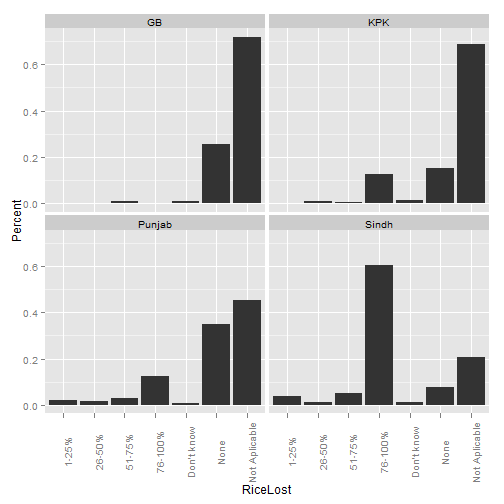
\includegraphics[width=.9\linewidth]{smallerDist/figures/fifteenDist} 
\end{knitrout}

\caption{Distribution for 15 Tehsils per Province.\label{fig:fifteenDist}}
\end{figure}

Now we wish to to look at the various distributions in a single plot.  Here is the code:
\begin{knitrout}
\definecolor{shadecolor}{rgb}{1, 1, 1}\color{fgcolor}\begin{kframe}
\begin{alltt}
\hlcomment{# plot distributions for all measurement sizes on same graph}
allT <- \hlfunctioncall{rbind}(rice5Perc, rice10Perc, rice15Perc, ricePerc)
allT$Size <- \hlfunctioncall{ordered}(allT$Size, levels = \hlfunctioncall{c}(5, 10, 15, \hlstring{"All"}))
\hlfunctioncall{ggplot}(allT, \hlfunctioncall{aes}(x = RiceLost, y = Percent)) + \hlfunctioncall{geom_bar}(\hlfunctioncall{aes}(group = Size, fill = Size), 
    stat = \hlstring{"identity"}, position = \hlstring{"dodge"}) + \hlfunctioncall{opts}(axis.text.x = \hlfunctioncall{theme_text}(angle = 90)) + 
    \hlfunctioncall{facet_wrap}(~Province)
\end{alltt}
\end{kframe}
\end{knitrout}


The plot is in Figure~\ref{fig:allDistInOne}.
\begin{figure}[!hbtp]
\begin{knitrout}
\definecolor{shadecolor}{rgb}{1, 1, 1}\color{fgcolor}\begin{kframe}


{\ttfamily\noindent\textcolor{warningcolor}{\#\# Warning: 'opts' is deprecated.\\\#\# Use 'theme' instead.\\\#\# See help("Deprecated")}}

{\ttfamily\noindent\textcolor{warningcolor}{\#\# Warning: 'theme\_text' is deprecated.\\\#\# Use 'element\_text' instead.\\\#\# See help("Deprecated")}}\end{kframe}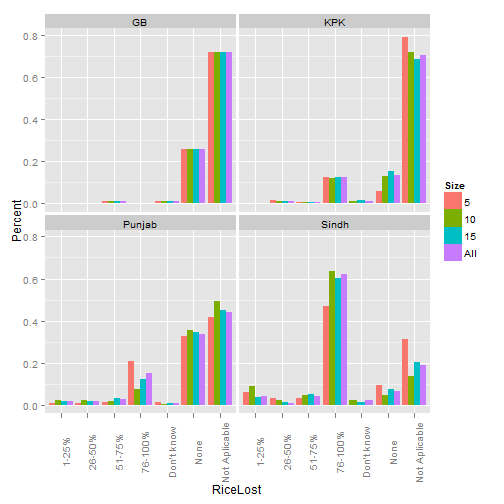
\includegraphics[width=.9\linewidth]{smallerDist/figures/allDistInOnePlot} 
\end{knitrout}

\caption{The distribution for all sampling types in one plot.\label{fig:allDistInOne}}
\end{figure}

Figure~\ref{fig:distErrors} displays the error between the smaller samples and the full distribution.  The code to do so is here:

\begin{knitrout}
\definecolor{shadecolor}{rgb}{1, 1, 1}\color{fgcolor}\begin{kframe}
\begin{alltt}
allC <- \hlfunctioncall{rbind}(compare5, compare10, compare15)
allC$Partial.Size <- \hlfunctioncall{ordered}(allC$Partial.Size, levels = \hlfunctioncall{c}(5, 10, 15))
allC$Province <- \hlfunctioncall{factor}(allC$Province)
\hlfunctioncall{ggplot}(allC, \hlfunctioncall{aes}(x = RiceLost, y = .Diff)) + \hlfunctioncall{geom_line}(\hlfunctioncall{aes}(fill = Province, 
    colour = Province, group = Province)) + \hlfunctioncall{opts}(axis.text.x = \hlfunctioncall{theme_text}(angle = 90)) + 
    \hlfunctioncall{facet_wrap}(~Partial.Size) + \hlfunctioncall{geom_hline}(yintercept = 0, colour = \hlstring{"grey"}, 
    linetype = 2)
\end{alltt}
\end{kframe}
\end{knitrout}


\begin{figure}[!hbtp]
\begin{knitrout}
\definecolor{shadecolor}{rgb}{1, 1, 1}\color{fgcolor}\begin{kframe}


{\ttfamily\noindent\textcolor{warningcolor}{\#\# Warning: 'opts' is deprecated.\\\#\# Use 'theme' instead.\\\#\# See help("Deprecated")}}

{\ttfamily\noindent\textcolor{warningcolor}{\#\# Warning: 'theme\_text' is deprecated.\\\#\# Use 'element\_text' instead.\\\#\# See help("Deprecated")}}\end{kframe}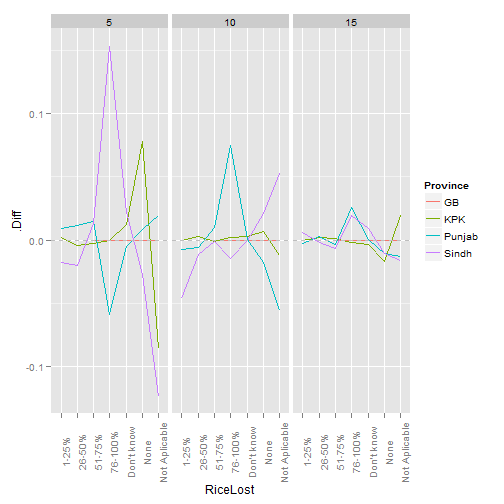
\includegraphics[width=.9\linewidth]{smallerDist/figures/distErrorsPlot} 
\end{knitrout}

\caption[Distribution Differences.]{The difference between the true distribution and the smaller smaples.\label{fig:distErrors}}
\end{figure}

Closing text.
